\chapter{METODE PENELITIAN}

\section{Jenis dan Rancangan Penelitian}
Isilah bagian ini dengan menjabarkan jenis dan rancangan penelitian yang Anda gunakan, dalam hal ini penelitian yang digunakan adalah penelitian kuantitatif.
\section{Lokasi Penelitian}
B
\section{Populasi dan Sampel Penelitian}
C
\section{Variabel Penelitian}
D
\section{Instrumen Penelitian}
E
\section{Teknik Pengumpulan Data}
F
\section{Teknik Analisis Data}
G
\section{Rencana Pelaksanaan}
Kegiatan penelitian ini akan mengikuti jadwal yang telah disusun pada~\ref{tab:kegiatan} berikut.

\begin{table}[h!]
	\centering
	\caption{Rencana Pelaksanaan Penelitian}
	\label{tab:kegiatan}
	\begin{tabular}{|l|llll|llll|llll|llll|}
		\hline
		\multicolumn{1}{|c|}{}                           & \multicolumn{4}{c|}{I}                                                                                                                                                                        & \multicolumn{4}{c|}{II}                                                                                                                                                  & \multicolumn{4}{c|}{III}                                                                                                                                                 & \multicolumn{4}{c|}{IV}                                                                                                                                                  \\ \cline{2-17} 
		\multicolumn{1}{|c|}{\multirow{-2}{*}{Kegiatan}} & \multicolumn{1}{c|}{1}                        & \multicolumn{1}{c|}{2}                        & \multicolumn{1}{c|}{3}                        & \multicolumn{1}{c|}{4}                        & \multicolumn{1}{c|}{1}                        & \multicolumn{1}{c|}{2}                        & \multicolumn{1}{c|}{3}                        & \multicolumn{1}{c|}{4}   & \multicolumn{1}{c|}{1}                        & \multicolumn{1}{c|}{2}                        & \multicolumn{1}{c|}{3}                        & \multicolumn{1}{c|}{4}   & \multicolumn{1}{c|}{1}                        & \multicolumn{1}{c|}{2}                        & \multicolumn{1}{c|}{3}                        & \multicolumn{1}{c|}{4}   \\ \hline
		Studi Literatur                                  & \multicolumn{1}{c|}{\cellcolor[HTML]{9B9B9B}} & \multicolumn{1}{c|}{\cellcolor[HTML]{9B9B9B}} & \multicolumn{1}{c|}{}                         & \multicolumn{1}{c|}{}                         & \multicolumn{1}{c|}{}                         & \multicolumn{1}{c|}{}                         & \multicolumn{1}{c|}{}                         & \multicolumn{1}{c|}{}    & \multicolumn{1}{c|}{}                         & \multicolumn{1}{c|}{}                         & \multicolumn{1}{c|}{}                         & \multicolumn{1}{c|}{}    & \multicolumn{1}{c|}{}                         & \multicolumn{1}{c|}{}                         & \multicolumn{1}{c|}{}                         & \multicolumn{1}{c|}{}    \\ \hline
		Pengambilan Data                                 & \multicolumn{1}{c|}{}                         & \multicolumn{1}{c|}{}                         & \multicolumn{1}{c|}{\cellcolor[HTML]{9B9B9B}} & \multicolumn{1}{c|}{\cellcolor[HTML]{9B9B9B}} & \multicolumn{1}{c|}{\cellcolor[HTML]{9B9B9B}} & \multicolumn{1}{c|}{\cellcolor[HTML]{9B9B9B}} & \multicolumn{1}{c|}{}                         & \multicolumn{1}{c|}{}    & \multicolumn{1}{c|}{}                         & \multicolumn{1}{c|}{}                         & \multicolumn{1}{c|}{}                         & \multicolumn{1}{c|}{}    & \multicolumn{1}{c|}{}                         & \multicolumn{1}{c|}{}                         & \multicolumn{1}{c|}{}                         & \multicolumn{1}{c|}{}    \\ \hline
		Pengolahan Data                                  & \multicolumn{1}{l|}{}                         & \multicolumn{1}{l|}{}                         & \multicolumn{1}{l|}{}                         &                                               & \multicolumn{1}{l|}{}                         & \multicolumn{1}{l|}{\cellcolor[HTML]{9B9B9B}} & \multicolumn{1}{l|}{\cellcolor[HTML]{9B9B9B}} & \cellcolor[HTML]{9B9B9B} & \multicolumn{1}{l|}{\cellcolor[HTML]{9B9B9B}} & \multicolumn{1}{l|}{}                         & \multicolumn{1}{l|}{}                         &                          & \multicolumn{1}{l|}{}                         & \multicolumn{1}{l|}{}                         & \multicolumn{1}{l|}{}                         &                          \\ \hline
		Analisis Data                                    & \multicolumn{1}{l|}{}                         & \multicolumn{1}{l|}{}                         & \multicolumn{1}{l|}{}                         &                                               & \multicolumn{1}{l|}{}                         & \multicolumn{1}{l|}{}                         & \multicolumn{1}{l|}{}                         &                          & \multicolumn{1}{l|}{\cellcolor[HTML]{9B9B9B}} & \multicolumn{1}{l|}{\cellcolor[HTML]{9B9B9B}} & \multicolumn{1}{l|}{\cellcolor[HTML]{9B9B9B}} & \cellcolor[HTML]{9B9B9B} & \multicolumn{1}{l|}{}                         & \multicolumn{1}{l|}{}                         & \multicolumn{1}{l|}{}                         &                          \\ \hline
		Penarikan Kesimpulan                             & \multicolumn{1}{l|}{}                         & \multicolumn{1}{l|}{}                         & \multicolumn{1}{l|}{}                         &                                               & \multicolumn{1}{l|}{}                         & \multicolumn{1}{l|}{}                         & \multicolumn{1}{l|}{}                         &                          & \multicolumn{1}{l|}{}                         & \multicolumn{1}{l|}{}                         & \multicolumn{1}{l|}{}                         & \cellcolor[HTML]{9B9B9B} & \multicolumn{1}{l|}{\cellcolor[HTML]{9B9B9B}} & \multicolumn{1}{l|}{\cellcolor[HTML]{9B9B9B}} & \multicolumn{1}{l|}{}                         &                          \\ \hline
		Penulisan Skripsi                                & \multicolumn{1}{l|}{}                         & \multicolumn{1}{l|}{}                         & \multicolumn{1}{l|}{}                         &                                               & \multicolumn{1}{l|}{}                         & \multicolumn{1}{l|}{}                         & \multicolumn{1}{l|}{}                         & \cellcolor[HTML]{9B9B9B} & \multicolumn{1}{l|}{\cellcolor[HTML]{9B9B9B}} & \multicolumn{1}{l|}{\cellcolor[HTML]{9B9B9B}} & \multicolumn{1}{l|}{\cellcolor[HTML]{9B9B9B}} & \cellcolor[HTML]{9B9B9B} & \multicolumn{1}{l|}{\cellcolor[HTML]{9B9B9B}} & \multicolumn{1}{l|}{\cellcolor[HTML]{9B9B9B}} & \multicolumn{1}{l|}{\cellcolor[HTML]{9B9B9B}} & \cellcolor[HTML]{9B9B9B} \\ \hline
	\end{tabular}
\end{table}

\begin{figure}[h!]
	\centering
	\tikzstyle{startstop} = [rectangle, rounded corners, minimum height=1cm, text centered, draw=black]
	\tikzstyle{io} = [trapezium, trapezium stretches=true, trapezium left angle=70,  trapezium right angle=110, minimum height=1cm, text centered]
	\tikzstyle{process} = [rectangle, minimum width=3cm, minimum height=1cm, text centered, draw=black]
	\tikzstyle{decision} = [diamond, minimum height=1cm, text centered, draw=black]
	\tikzstyle{arrow} = [ultra thick,->,>=stealth]
	
	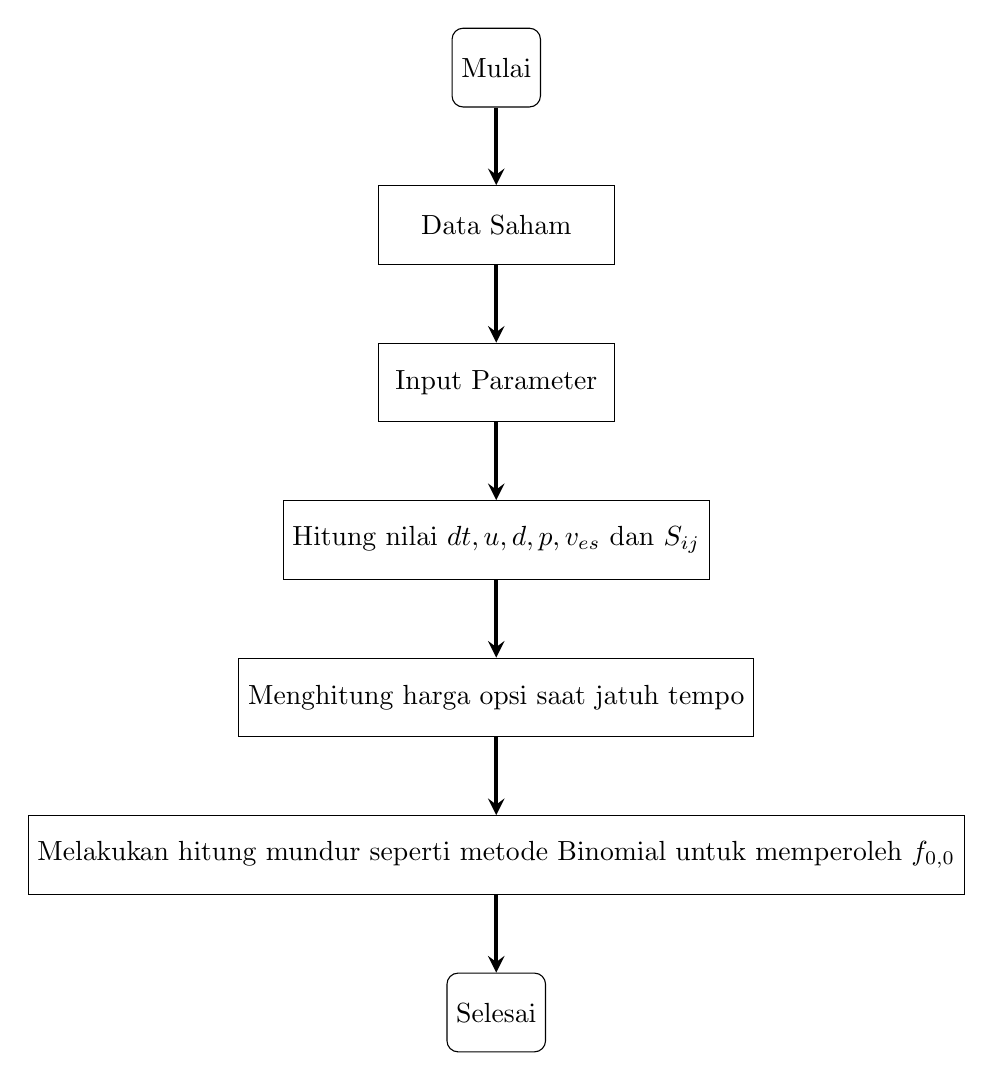
\begin{tikzpicture}[node distance=2cm]
		\node (start) [startstop] {Mulai};
		\node (pro1) [process, below of=start] {Data Saham};
		\node (pro2) [process, below of=pro1] {Input Parameter};
		\node (pro3) [process, below of=pro2] {Hitung nilai $dt, u, d, p, v_{es}$ dan $S_{ij}$};
		\node (pro4) [process, below of=pro3] {Menghitung harga opsi saat jatuh tempo};
		\node (pro5) [process, below of=pro4] {Melakukan hitung mundur seperti metode Binomial untuk memperoleh $f_{0,0}$};
		\node (stop) [startstop, below of=pro5] {Selesai};
			
		\draw [arrow] (start) -- (pro1);
		\draw [arrow] (pro1) -- (pro2);
		\draw [arrow] (pro2) -- (pro3);
		\draw [arrow] (pro3) -- (pro4);
		\draw [arrow] (pro4) -- (pro5);
		\draw [arrow] (pro5) -- (stop);		
	\end{tikzpicture}
\caption{Alur penelitian}
\end{figure}
